% !TEX root = ../main.tex
\lecture{8}{2026-11-04}{Marketingprogramm III}

\subsection{Marketingprozess III: Marketingprogramm }

\subsubsection{Produktdimensionen}
\begin{enumerate}
    \item Kernprodukt (Inhalt)
    \item Reales Produkt (Form)
    \begin{itemize}
        \item Markenname
        \item Verpackung
        \item Qualität
        \item Design
        \item Produktfunktionalität
    \end{itemize}
    \item Erweitertes Produkt (zusätzliche Dienstleistungen)
    \begin{itemize}
        \item Kundendienst
        \item Kostenlose Goodies
    \end{itemize}
\end{enumerate}
\subsubsection{7Ps im Dienstleistungsmarketing}
Hauptproblematik bei Dienstleistungen: Erst nach dem die Leistung erbracht wurde, kann der Kunde die Qualität beurteilen, was zu Vorsicht beim Kaufen führt.
\begin{itemize}
    \item Neben den 4Ps(Product, Price, Placement,Promotion)
    \begin{itemize}
        \item Person, die die Leistung erbringt (gepflegtes aussehen, professionalität)
        \item Physikalische Umgebung (Ambiente)
        \item Prozess 
    \end{itemize}
\end{itemize}
\subsubsection{Produktzyklus}
 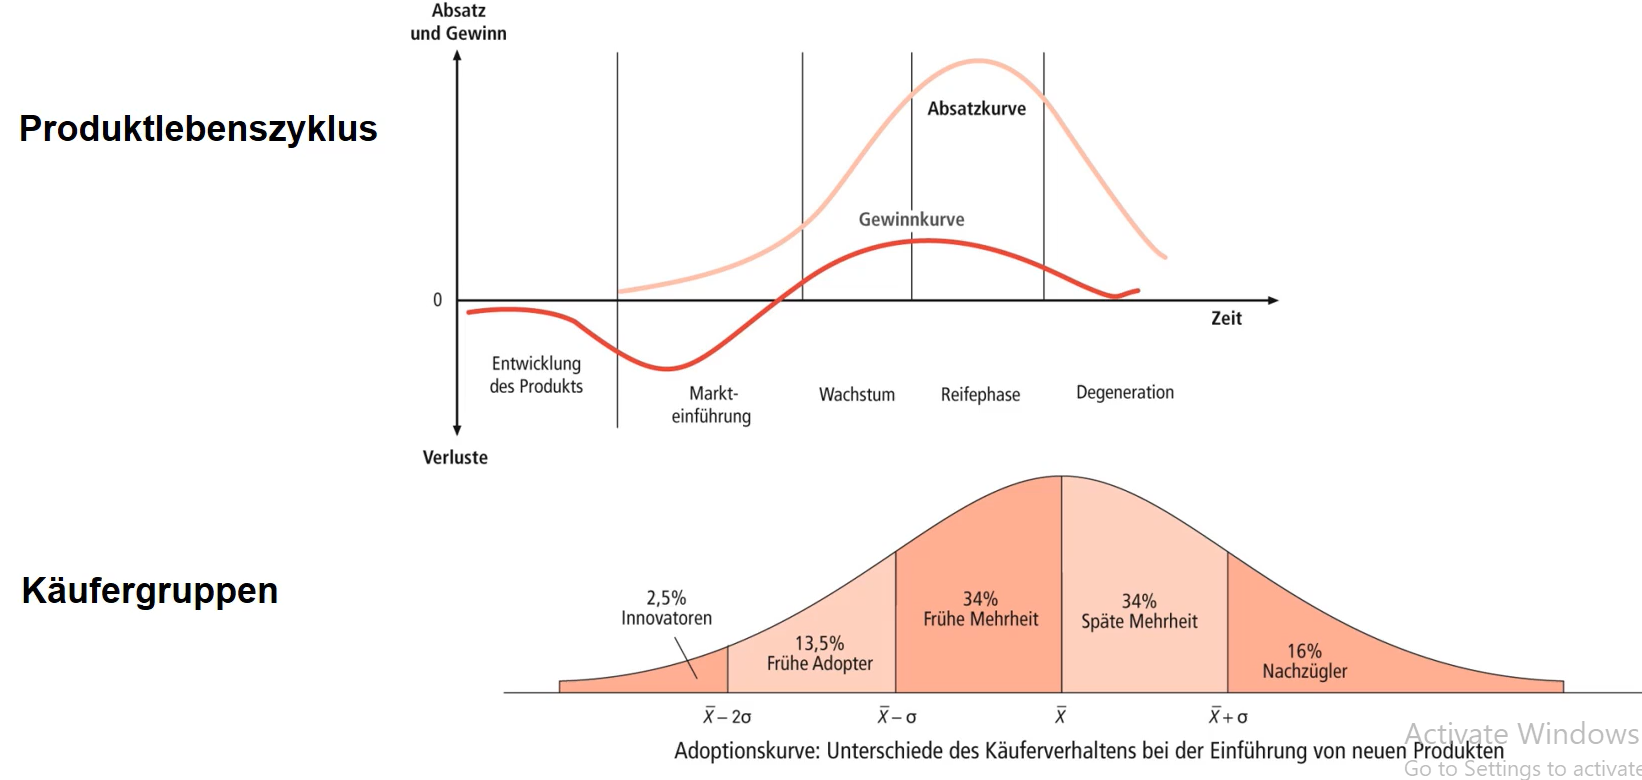
\includegraphics[width=\textwidth,height=0.7\textheight,keepaspectratio]{figures/Marketing_Prodcycle.png}

 \pagebreak
\subsubsection{Produktlinie}
\begin{definition}
    [Produktlinie] ist eine Gruppe von Produkten, die konvergente Nutzen, ähnliche Preise oder Käufer verbunden sind. \textbf{Kernentscheidung:} über die Länge einer Produktlinie, wie viele ähnliche Produkte mit Preis oder Qualitätsklassen eine Marke haben soll
\end{definition}

\begin{definition}
    [Markenkannibalismus] die Problematik intern konkurrierender Produkte, was Entscheidungen bezüglich der Budget-Allokation erschwert 
\end{definition}

\subsubsection{Markenpositionierung}
\begin{itemize}
    \item Funktionale: Konkret, sachlich auf Produkteingenschaften bezogen, Differenzierbar
    \item Emotionale:
    \begin{itemize}
        \item Abstrakter Nutzen
        \item Erlaubt für Differenzierung in homogenen Produktmärkten
        \item Stiftet Identität
        \item Keine Überprüfbarkeit
        \item Geringe Rationale Aspekte (führt zur Hinterfragung des Produkts)
    \end{itemize}
    \item Markenclaim
    \begin{itemize}
        \item Checklist zur Überprüfung der Eignung der Marke an Kundenmotive/bedürfnisse
        \begin{itemize}
            \item Markenclaim: kurz, prägnant
            \item Unique Selling Proposition überzeugend?
            \item Glaubwürdigkeit
            \item Welche emotionalen und rationalen Benefits bietet die Marke?
        \end{itemize}
    \end{itemize}
\end{itemize}

\subsubsection{Erfahrungskurve}
\begin{itemize}
    \item Beschreibt die Kostenreduktion abhängig der kumulativen Produktionsmenge
    \item Effizienz-Steigerung 
    \item Verteilung der Kosten auf höheren Stückzahl
\end{itemize}

\pagebreak
\subsubsection{Preisstrategien: Marktabschöpfungsstrategie }
    \begin{itemize}
        \item Preise werden anfänglich hoch gesetzt um an Kunden mit hoher Zahlungsfähigkeit gezielt zu verkaufen
        \item Mit der Zeit werden Preise gesenkt, sodass andere Zahlungsbereitschaften abgeschöpft werden können
        \item \textbf{Begünstigt durch:} 
        \begin{itemize}
            \item Hohe Image
            \item Hohe Zahlungsbereitschaft zahlreicher Kunden
            \item Nicht schnell imitierbar
        \end{itemize}
    \end{itemize}

\subsubsection{Preisstrategien: Penetrationspreis oder Marktdurchdringung}

\begin{itemize}
    \item Vom Anfang an Skalen-Effekt für niedrige Stückpreise. 
    \item Oft anfänglich bei Verlust verkaufen
    \item Aus der Konkurrenz Anteil gewinnen
    \item  \textbf{Begünstigt durch:}
    \begin{itemize}
        \item Starke Preissensibilität (elastizität)
        \item Hohe Produktivität, grosse Kapitalmengen
        \item Konkurrenz nicht fähig zum niedrigeren Preis zu verkaufen
    \end{itemize}
    
\end{itemize}

\subsubsection{Reaktionsstrategien bei Preisänderungen}
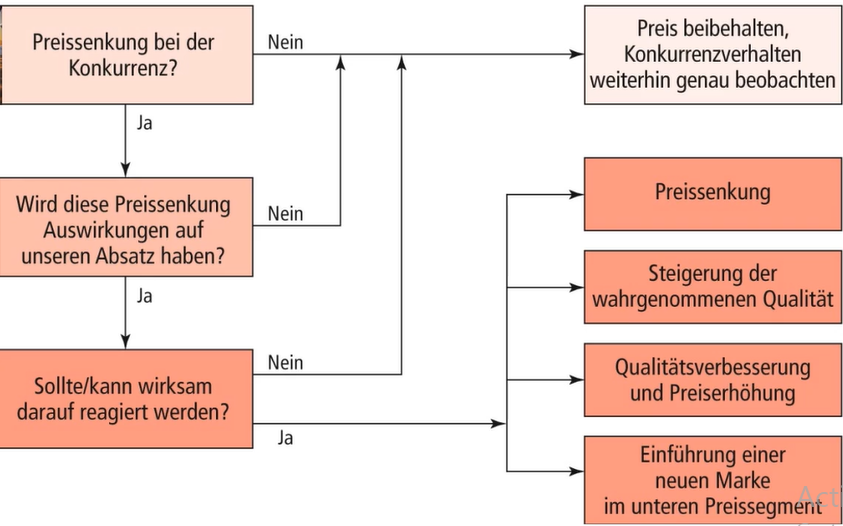
\includegraphics[width=\textwidth,height=0.7\textheight,keepaspectratio]{figures/PreisReaktion.png}